\let\negmedspace\undefined
\let\negthickspace\undefined
\documentclass[journal]{IEEEtran}
\usepackage[a5paper, margin=10mm, onecolumn]{geometry}
%\usepackage{lmodern} % Ensure lmodern is loaded for pdflatex
\usepackage{tfrupee} % Include tfrupee package

\setlength{\headheight}{1cm} % Set the height of the header box
\setlength{\headsep}{0mm}     % Set the distance between the header box and the top of the text

\usepackage{gvv-book}
\usepackage{gvv}
\usepackage{cite}
\usepackage{amsmath,amssymb,amsfonts,amsthm}
\usepackage{algorithmic}
\usepackage{graphicx}
\usepackage{textcomp}
\usepackage{xcolor}
\usepackage{txfonts}
\usepackage{listings}
\usepackage{enumitem}
\usepackage{mathtools}
\usepackage{gensymb}
\usepackage{comment}
\usepackage[breaklinks=true]{hyperref}
\usepackage{tkz-euclide} 
\usepackage{listings}
% \usepackage{gvv}                                        
\def\inputGnumericTable{}                                 
\usepackage[latin1]{inputenc}                                
\usepackage{color}                                            
\usepackage{array}                                            
\usepackage{longtable}                                       
\usepackage{calc}                                             
\usepackage{multirow}                                         
\usepackage{hhline}                                           
\usepackage{ifthen}                                           
\usepackage{lscape}
\usepackage{circuitikz}
\usepackage[utf8]{inputenc}   
\usepackage[T1]{fontenc}      
\usepackage{amsmath}          

\tikzstyle{block} = [rectangle, draw, fill=blue!20, 
    text width=4em, text centered, rounded corners, minimum height=3em]
\tikzstyle{sum} = [draw, fill=blue!10, circle, minimum size=1cm, node distance=1.5cm]
\tikzstyle{input} = [coordinate]
\tikzstyle{output} = [coordinate]




\bibliographystyle{IEEEtran}
\vspace{3cm}

\title{5.7.12}
\author{AI25BTECH11039-Harichandana Varanasi}
 \maketitle
% \newpage
% \bigskip
{\let\newpage\relax\maketitle}

\renewcommand{\thefigure}{\theenumi}
\renewcommand{\thetable}{\theenumi}
\setlength{\intextsep}{10pt} % Space between text and floats


\numberwithin{equation}{enumi}
\numberwithin{figure}{enumi}
\renewcommand{\thetable}{\theenumi}



\date{}

\begin{document}
\maketitle


\textbf{Question:}
If 
\[
\vec{A}=\myvec{4 & 2\\ -1 & 1},
\]
show that $(\vec{A}-2\vec{I})(\vec{A}-3\vec{I})=\vec{0}$.


\begin{solution}
\renewcommand\theequation{\arabic{equation}}
\setcounter{equation}{0}

From the characteristic equation definition and the \text{Cayley-Hamilton} theorem,
\[
f(\lambda)=\det(\vec{A}-\lambda\vec{I})=0,\qquad f(\vec{A})=\vec{0}.
\]
For the given matrix,
\begin{align}
\det(\vec{A}-\lambda\vec{I})
&=\det\myvec{4-\lambda & 2\\ -1 & 1-\lambda}
=(4-\lambda)(1-\lambda)-(-2) \nonumber\\
&=\lambda^2-5\lambda+6
=(\lambda-2)(\lambda-3).
\label{eq:char}
\end{align}
Hence, by  \text{Cayley-Hamilton},
\begin{align}
f(\vec{A})
&=\vec{A}^2-5\vec{A}+6\vec{I}
=(\vec{A}-2\vec{I})(\vec{A}-3\vec{I})
=\vec{0}.
\label{eq:CH}
\end{align}

\end{solution}


                     
\begin{figure}[H]
  \centering
  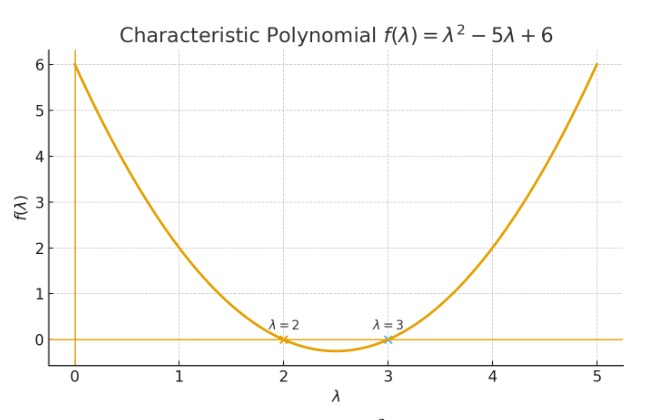
\includegraphics[width=0.8\linewidth]{figs/matgeo-5.7.12.jpeg}
  \caption{Characteristic polynomial $f(\lambda)=\lambda^2-5\lambda+6$ with roots $\lambda=2,3$.}
\label{fig:charpoly-A}
\end{figure}

 
\end{document}
